%% Based on a TeXnicCenter-Template by Tino Weinkauf.
%%%%%%%%%%%%%%%%%%%%%%%%%%%%%%%%%%%%%%%%%%%%%%%%%%%%%%%%%%%%%

%%%%%%%%%%%%%%%%%%%%%%%%%%%%%%%%%%%%%%%%%%%%%%%%%%%%%%%%%%%%%
%% HEADER
%%%%%%%%%%%%%%%%%%%%%%%%%%%%%%%%%%%%%%%%%%%%%%%%%%%%%%%%%%%%%
\documentclass[a4paper,oneside,12pt]{report}
% Alternative Options:
% Paper Size: a4paper / a5paper / b5paper / letterpaper / legalpaper / executivepaper
% Duplex: oneside / twoside
% Base Font Size: 10pt / 11pt / 12pt


\usepackage[utf8]{inputenc} % Encodage utf-8
\usepackage[T1]{fontenc} % Nouvelle norme pour codage des caractères
\usepackage{aeguill}

%Pour faire une page landscape
\usepackage{lscape}

% pour l'ajout des "liste" dans la table des matières
\usepackage[nottoc]{tocbibind}
\usepackage[top=2.5cm, bottom=2.5cm, left=2cm , right=2cm]{geometry}

% en-tête et pied de page
\usepackage{fancyhdr}
 
\usepackage[frenchb]{babel} % Règles typographiques françaises, césures
\usepackage{graphicx} % Insertion images
\usepackage{epstopdf} % Converit les images .eps en .pdf pour la compilation avec pdflatex

% package pour tous ce qui est math
\usepackage{amsmath}
\usepackage{amssymb}
\usepackage{amsthm}

\usepackage[colorlinks=true, linkcolor=blue, citecolor=blue]{hyperref}
\usepackage{listings} %Insertion de code dans le fichier
\lstset{
language=C,
basicstyle=\footnotesize,
numbers=left,
numberstyle=\normalsize,
numbersep=7pt,
}


%% Packages for Graphics & Figures %%%%%%%%%%%%%%%%%%%%%%%%%%
\usepackage{graphicx} %%For loading graphic files


%% Math Packages %%%%%%%%%%%%%%%%%%%%%%%%%%%%%%%%%%%%%%%%%%%%
\usepackage{amsmath}
\usepackage{amsthm}
\usepackage{amsfonts}

% Titre
\newcommand{\RapportTitre}{Inkcut for Inkscape}     

% la date
\newcommand{\RapportDate}{\today}   

% Departement
\newcommand{\RapportDepartement}{Technologies Industrielles (TIN)}    
\newcommand{\RapportOrientation}{Electronique et Automatisation Industrielle (EAI)}

% FabLab
\newcommand{\RapportEcole}{\href{http://www.heig-vd.ch/}{HEIG-VD}}      
\newcommand{\RapportLogoFabLab}{\href{http://www.heig-vd.ch/}{
\includegraphics[height=4cm]{imgs/fablab_logo_11.png}}}

%%%%%%%%%%%%%%%%%%%%%%%%%%%%%%%%%%%%%%%%%%%%%%%%%%%%%%%%%%%%%
%% DOCUMENT
%%%%%%%%%%%%%%%%%%%%%%%%%%%%%%%%%%%%%%%%%%%%%%%%%%%%%%%%%%%%%
\begin{document}


\begin{center}
	\RapportLogoFabLab \hfill
\end{center}

\vspace{1cm}
\noindent \hrulefill
\begin{center}
%titre en gras
\huge \RapportTitre
\end{center}
\noindent \hrulefill

\begin{center}
\Large Extension pour gérer les plotters du Fablab Fribourg
\end{center}

\vspace{\fill}
\vspace{\fill}

\begin{flushleft}
	\begin{tabular}{l l}
		Auteur : &Dylan Collaud\\
		Mail : &dylan.collaud@gmail.com\\
		Inkscape : &testé sur 0.48.5 et 0.91\\
		Date : &21.08.2015\\
	\end{tabular}

\end{flushleft}

\vspace{\fill}

\pagestyle{empty} %No headings for the first pages.

%% Inhaltsverzeichnis %%%%%%%%%%%%%%%%%%%%%%%%%%%%%%%%%%%%%%%
\tableofcontents %Table of contents
\cleardoublepage %The first chapter should start on an odd page.

\pagestyle{plain} %Now display headings: headings / fancy / ...



%% Chapters %%%%%%%%%%%%%%%%%%%%%%%%%%%%%%%%%%%%%%%%%%%%%%%%%

%%%%%%%%%%%%%%%%%%%%%%%%%%%%%%%%%%%%%%%%%%%%%%%%%%%%%%%%%%%%%

\chapter{Introduction}\label{Intro}

\section{Inkscape}\label{Inkscape}
Inkscape est un logiciel open source qui permet de créer des dessins vectoriels. Celui-ci est souvent utilisé au sein du FabLab
pour la découpe avec la laser. Ce logiciel n'est pas visuellement attractif, mais il possède énormément de fonctionnalités.



\section{InkCut}\label{InkCut}
InkCut est une extension en python pour le logiciel Inkscape. Celui-ci permet de commander les plotters disponibles au FabLab.
InkCut est une extension stable, mais qui a d'abord été créée pour Linux, celle-ci fonctionne sur Windows, mais elle a besoin de quelques adaptations
qui seront décrites dans la suite de ce document.

\section{Choix d'installation}
Dans la suite de ce document, vous aurez la possibilité d'installer cette extension pour windows ou linux (pas encore disponible).

\begin{enumerate}

\item \nameref{windowsRapide}
\item \nameref{linux}

\end{enumerate}


%%%%%%%%%%%%%%%%%%%%%%%%%%%%%%%%%%%%%%%%%%%%%%%%%%%%%%%%%%%%%

\chapter{Installation InkCut sur Windows version rapide FabLab}\label{windowsRapide}

L'installation de InkCut a été testée sur InkScape 0.48.5 et 0.91. La version n'est pas très importante, mais c'est toujours mieux d'avoir la dernière version
du logiciel. Inkscape est téléchargeable sur leur \href{https://inkscape.org/fr/telechargement/}{site officiel}.
Si vous avez déjà une version d'inkscape, vous n'avez rien besoin de faire.

\section{Dossier à copier}
Vous pouvez trouver le dossier contenant l'extension sur les serveurs du FabLab ou sur une clé usb au FabLab. Récupérer le dossier "inkscape" et copiez-le dans votre dossier "Program Files". Les fichiers nécessaires et l'extension Inkcut sera automatiquement ajoutée.\newline

Dès que vous avez copié ce dossier, vous avez fini l'installation et vous pouvez passer à la partie : \nameref{inkcut}.

%%%%%%%%%%%%%%%%%%%%%%%%%%%%%%%%%%%%%%%%%%%%%%%%%%%%%%%%%%%%%

%%%%%%%%%%%%%%%%%%%%%%%%%%%%%%%%%%%%%%%%%%%%%%%%%%%%%%%%%%%%%

\chapter{Installation InkCut sur Linux}\label{linux}

Si une personne est motivée a mettre en place sur linux, n'hésitez pas à me contacter : dylan.collaud@gmail.com

\section{Téléchargement}

\section{Installation}

\section{Modification}

%%%%%%%%%%%%%%%%%%%%%%%%%%%%%%%%%%%%%%%%%%%%%%%%%%%%%%%%%%%%%

%%%%%%%%%%%%%%%%%%%%%%%%%%%%%%%%%%%%%%%%%%%%%%%%%%%%%%%%%%%%%

\chapter{Utilisation InkCut}\label{inkcut}

\section{Modèle de base}

Pour l'exemple d'utilisation, il faut utiliser un simple modèle quelconque de type carré ou rond. Pour se faire, utiliser l'outil F4 ou F5.\\

Dès que vous avez votre forme, il faut obligatoirement la transformer en 'Objet en chemin' dans le menu 'Chemin'. Dès que votre objet, texte ou autre est prêt,
vous pouvez passer à l'étape suivante.

\section{Utilisation de l'extension}
L'extension est utilisable dans le menu 'Extension', 'Cutter/plotter', 'InkCut'. Pour l'utiliser, il faut sélectionner votre forme et cliquer sur InkCut.
Vous devriez obtenir un résultat comme le suivant : 

\begin{figure}[h]
 \begin{center}
  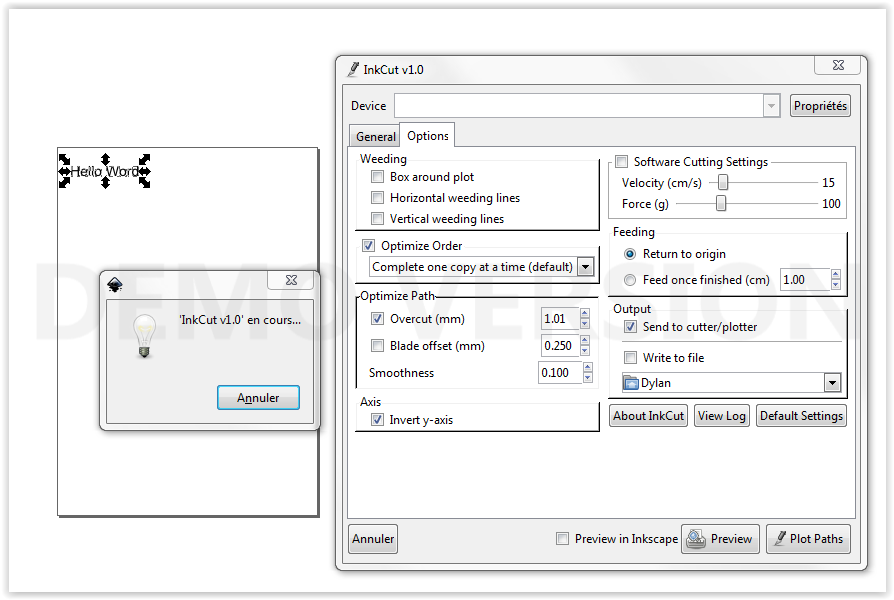
\includegraphics[width=13cm]{imgs/inkcut.png}
  \caption{ Interface extension InkCut }
 \end{center}
\end{figure}
\newpage
Vous pouvez accèder aux paramêtres de communication avec le bouton 'Propriété'. Une nouvelle fenêtre s'ouvre et vous pouvez sélectionner
le port com de communication dans la photo ci-dessous vous voyez le port com 3.

\begin{figure}[h]
 \begin{center}
  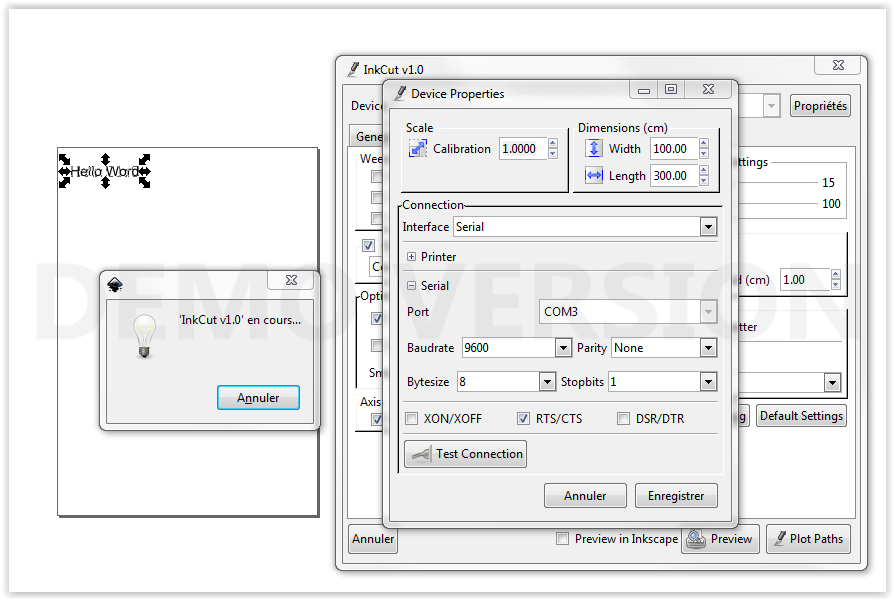
\includegraphics[width=15cm]{imgs/inkcutParam.png}
  \caption{ Paramêtre de communication InkCut }
 \end{center}
\end{figure}

Comme on le voit dans la prise d'écran ci-dessus, il faut sélectionner la case RTS/CTS seulement. 
Les autres paramètres n'ont pas besoin d'être modifiés. Dès que c'est fait, vous pouvez enregistrer les paramètres et lancer un test pour vérifier le bon fonctionnement.
Vous pouvez sans autre lancer la découpe. Si vous avez eu des problèmes lors des manipulations, référez-vous à la partie suivante.

\newpage
\section{Bug possible}

\subsection{Erreur : type Path}

\begin{figure}[h]
 \begin{center}
  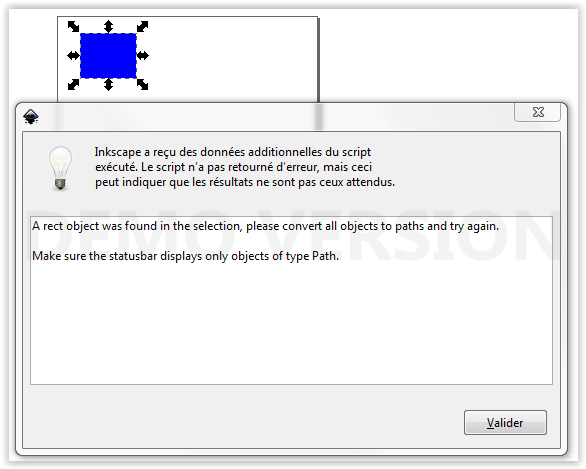
\includegraphics[width=15cm]{imgs/inkcutErrorPath.png}
  \caption{ Erreur type Path  }
 \end{center}
\end{figure}

\textbf{Solution :} Il s'agit d'un problème lié au chemin de votre forme. Celle-ci doit être convertie en chemin. 
Pour ce faire aller dans le menu 'chemin' puis 'Objet en chemin'.
\newpage

\subsection{Erreur : Texte}
\begin{figure}[h]
 \begin{center}
  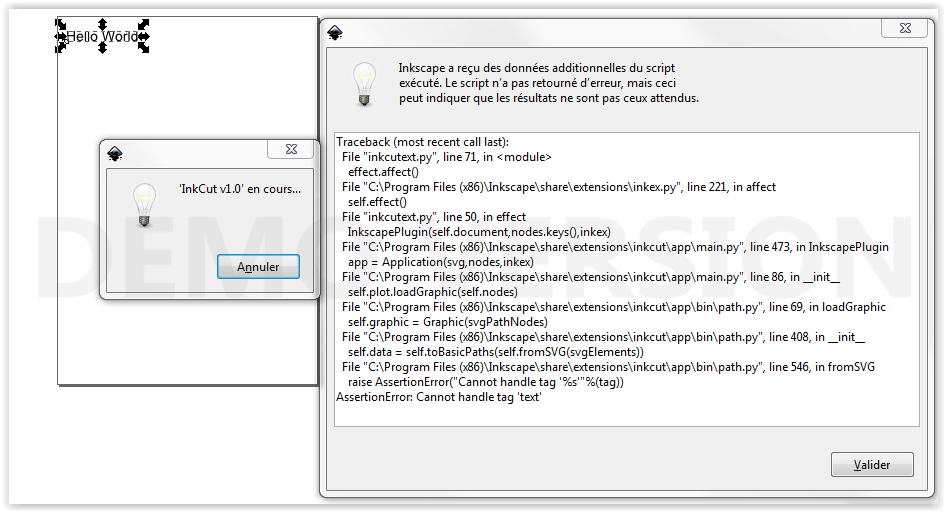
\includegraphics[width=15cm]{imgs/inkcutErrorText.png}
  \caption{ Erreur Texte  }
 \end{center}
\end{figure}

\textbf{Solution :} Comme dans le précédent bug, le texte n'est pas en chemin. Pour corriger le problème, il faut aller dans le menu 'chemin'
puis 'Objet en chemin'.
\newpage


\subsection{Erreur : forme groupée}
\begin{figure}[h]
 \begin{center}
  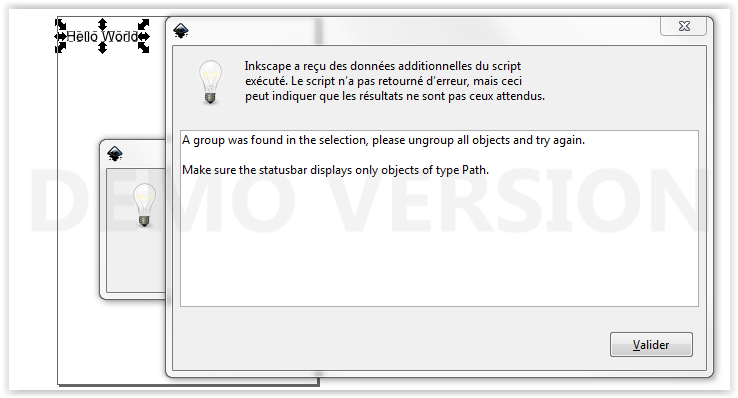
\includegraphics[width=15cm]{imgs/inkcutErrorGroup.png}
  \caption{ Erreur forme groupée }
 \end{center}
\end{figure}

\textbf{Solution :} Cette erreur peut arriver si vous importez des fichiers vectoriels ou avec du texte. Il vous suffit de faire un clic droit sur l'image puis 'dégrouper'.
\newpage

\subsection{Erreur : inconnu}

Pour toutes erreur inconnu survenant lors de l'utilisation, vous pouvez m'envoyer un mail à l'adresse : dylan.collaud@gmail.com afin que je puisse la résoudre et l'ajouté à ce document. Afin que j'ai toute les informations, merci de me décrire et m'envoyer précisément l'erreur : \\

\begin{itemize}
	\item Capture d'écran de l'erreur comme ci-dessus ou copy du texte d'erreur
	\item Si possible le modèle/fichier SVG que je puisse tester sur mon ordinateur
	\item divers modifications que vous auriez apportées dans les fichiers Inkscape
\end{itemize}

\newpage
\chapter{Conclusion}
J'espère que ce document vous permettra d'utiliser convenablement les découpeuses vinyle du Fablab. Je rajoute volontiers la partie linux si quelqu'un m'indique comment faire une installation simple et efficace comme pour windows.\\


%%%%%%%%%%%%%%%%%%%%%%%%%%%%%%%%%%%%%%%%%%%%%%%%%%%%%%%%%%%%%

%%%%%%%%%%%%%%%%%%%%%%%%%%%%%%%%%%%%%%%%%%%%%%%%%%%%%%%%%%%%%
%% BIBLIOGRAPHY AND OTHER LISTS
%%%%%%%%%%%%%%%%%%%%%%%%%%%%%%%%%%%%%%%%%%%%%%%%%%%%%%%%%%%%%
%% A small distance to the other stuff in the table of contents (toc)
\addtocontents{toc}{\protect\vspace*{\baselineskip}}

%% The Bibliography
%% ==> You need a file 'literature.bib' for this.
%% ==> You need to run BibTeX for this (Project | Properties... | Uses BibTeX)
%\addcontentsline{toc}{chapter}{Bibliography} %'Bibliography' into toc
%\nocite{*} %Even non-cited BibTeX-Entries will be shown.
%\bibliographystyle{alpha} %Style of Bibliography: plain / apalike / amsalpha / ...
%\bibliography{literature} %You need a file 'literature.bib' for this.


%%%%%%%%%%%%%%%%%%%%%%%%%%%%%%%%%%%%%%%%%%%%%%%%%%%%%%%%%%%%%
%% APPENDICES
%%%%%%%%%%%%%%%%%%%%%%%%%%%%%%%%%%%%%%%%%%%%%%%%%%%%%%%%%%%%%
\appendix
%% ==> Write your text here or include other files.

%\input{FileName} %You need a file 'FileName.tex' for this.


\end{document}

